\documentclass{article}
\usepackage{graphics}
\usepackage{indentfirst}
\usepackage{amsmath}
\usepackage{algorithm}
\usepackage{algorithmic}
\usepackage{bm}
\usepackage{setspace}
\usepackage{graphicx}
\usepackage{float}
\usepackage{CJKutf8}
\author{Ruichen Wang}
\title{Basis}

\begin{document}
\begin{CJK*}{UTF8}{gbsn}
\maketitle
\centerline{\textbf{Some Basics}}
C4.5, ID3, CART, K-means, SVM, Kernel function, SMO, EM, Naive bayes, Variational inference, PageRank, Adaboost, KNN, Data cleaning, Linear regression, Logistic regression, LDA, PCA, Random Forest, Bagging \& stacking, Softmax, GBDT, Xgboost, LightGBM, PCA, Max-entorpy, Gradient diminishing, FM, LFM, MF, SVD, SVD++, Simhash, Max likelihood, ALS, L1 norm, L2 norm, Discriminate \& Generative model, Entorpy, Cross-entropy, KL divergence, SGD, BGD, MBGD, Adam, Newton's method, Unbiased estimator, F1 score, Recall, Prercision, AUC, ROC, Cross validation, Bias-Variance tradeoff, Loss function, Overfitting \& underfitting, DBSCAN, TF-IDF, Text rank, Word2vec, Glove, Fast-text, Collaborative Filtering, User-cf, Item-cf, Dropout, Batch norm, Maxpooling, Avg pooling, Global avg pooling, Respective field, LR normalization, Online learning, FTRL, FOBOS, RDA, Tree row \& column sampling,  ANN, Tree normalization, RNN, LSTM, GRU, CRF, RNN \& CNN, KDtree, Resnet, Seq2seq, Deep wise CNN, 1X1 kernel, SVM multi-classification, Attention, Conv complexity, Pearson correlation, Gibbs sampling, t-SNE, Learning to Rank, mAP, NDCG, Hash.

\centerline{\rule{\textwidth}{1pt}}

\section{ID3, C4.5, CART difference?}
What is Decision Tree (DT)? \\
DTs are non parametric superivised learning method, can be used for classification and regression. DTs need little data preparation. No need NOrmalization. White box model. Easily overfitting, sensitive to variation, because may build complete different trees, can be mitigated by using ensemble. Based on greedy opt to solve NP-complete problem, may reach local optimal. Need balance dataset. \\
\begin{figure}[H]
\centering
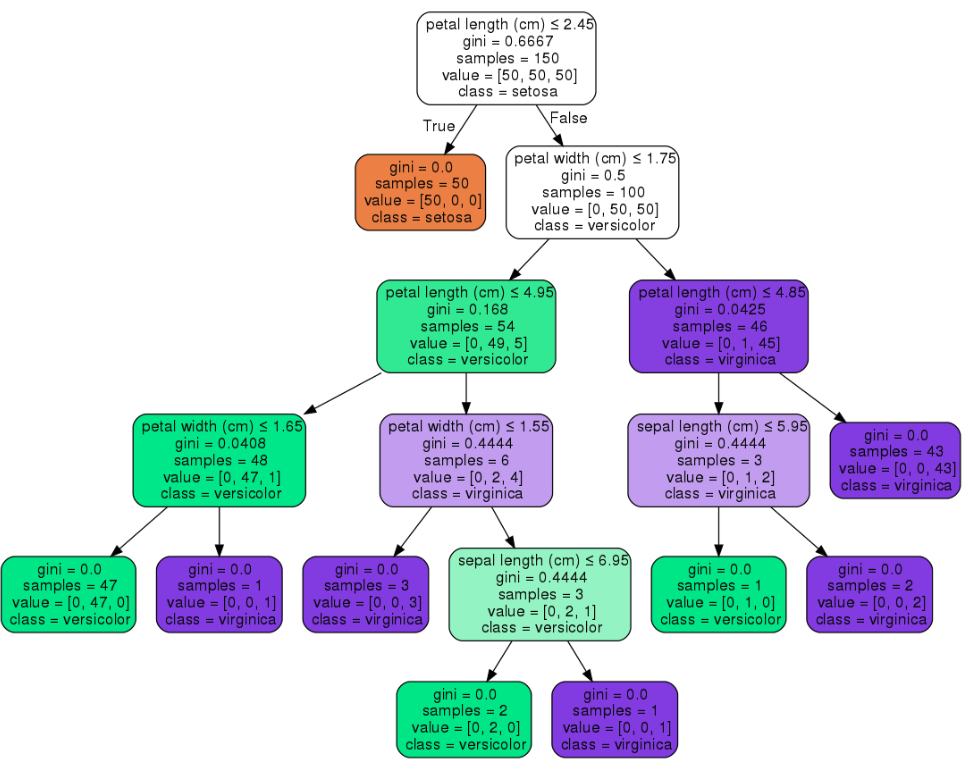
\includegraphics[width=4in,height=3in]{dt}
\caption{A decision tree using gini.}
\end{figure} 

Pratical Tips:
\begin{itemize}
\item DT tend overfit if using a large number of features, Using a ratio to sample the features.
\item Consider perform feature dimensionality reduction (PCA, Feature selection).
\item Control max depth, control min samples per leaf to prevent overfitting
\end{itemize}
ID3 (info gain) \\
\textbf{Entropy $H(S)$} is a measure of uncertainty of data. 
$$H(S)=\sum_{x \in S}-p(x)logp(x)$$
\textbf{Information Gain $IG(S)$} is a measure of differenece in entropy before and after $S$ splited on attribute A.
$$IG(S,A)=H(S)-\sum_{t \in A}p(t)H(t)=H(S)-H(S|A)$$
C4.5 (gain ratio)
C4.5 is the successor to ID3. Can handle continuous attribute.
$$GainRatio(S,A)=\frac{IG(S,A)}{IV(A)}$$
CART(Gini impurity)
CART using binary split, Split based on one variable. Pruning mainly has two types : pre and post. CART use CCP (cost complexity pruning), which is defined by $\frac{error rate}{tree complexity}$
$$Gini(A,S)=1-\sum_{t \in A} p_{t}^{2}$$


\section{Why L1 regulation generates sparsity? L2 regulation cause blur?}

Firstly, why do we want the result matrix to be sparse?

Consider 1 million dimension, calculate the inner product between $w$ and $x$ need a lot of computation. If the $w$ can be sparse, the inner product will only be performed on the non-zero columns.

Or consider another situation, in some scenario, there are free data and many features, which is often called as \textbf{`small n, large p problem'}. If $n \ll p $, then our model will be very complex, our $w$ will be a singular matrix ($|w|=0$). In other words, \textbf{overfitting}.

One way to control overfitting is adding a regularization term to the loss function. Rigde  ($l_{2} norm$) and LASSO ($l_{1} norm$) regression are two very common regression ways.
$$J(w)=Loss(x)+\lambda ||w||_{2}^{2}$$
$$J(w)=Loss(x)+\lambda ||w||_{1}$$
Assume we use loss using MSE, the target function can also be denoted as :
$$ \mathop{\min}_{w} \frac{1}{n}||y-Xw||^{2} \quad  s.t. \lambda ||w||_{2}^{2} \leq C $$
$$ \mathop{\min}_{w} \frac{1}{n}||y-Xw||^{2} \quad  s.t. \lambda ||w||_{1} \leq C $$

Back to the problem, intuitivly, the target loss will alway intersect at the coordinate axis when using l1 norm. Imaging high dimension situation, the angles will certainly more likely to be intersected, while the ball will not.

\begin{figure}[H]
\centering
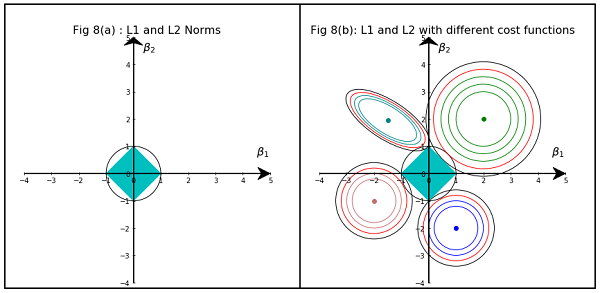
\includegraphics[width=3.5in,height=1.7in]{l1l2}
\caption{L1 and L2 norm.}
\end{figure}

For more math proof, see \textit{http://freemind.pluskid.org/machine-learning/sparsity-and-some-basics-of-l1-regularization}

\paragraph{Why L2 regulation cause blur?}

In generative models, eg.VAE, L2 norm / L2 loss / MSE tend to yield blurry images. We try to explain this in probabilistic settings. In Gaussian distribution, it defines as :
$$p(x|\mu,\sigma^{2})=\frac{1}{Z}exp\left( -\frac{||\mu-x||^{2}}{2\sigma^{2}}\right)$$
$$logp(x|\mu,\sigma^{2}) \propto exp\left(-\frac{1}{2}||x_{\mu}-x||^{2}  \right)$$
As we can see, minimizing MSE, is same as maximizing the log likelihood of gaussian, we make the assumption that our $x$ comes from a gaussian.


\begin{figure}[H]
\centering
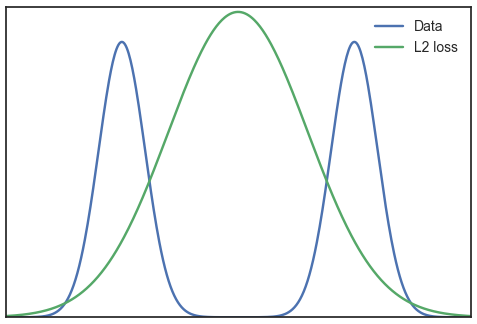
\includegraphics[width=3in,height=1.7in]{l2}
\caption{Gaussian and multinomial.}
\end{figure}

In reality, there often many hidden variables (multinomial) controls the $x$. A simple example, we have white and black dogs as dataset $x$. maximizing the likelihood will blur the two and generate gray dogs.

\section{One-hot encoding for gbdt?}

It is often the case that we have continuous and categorical features. One-hot encoding may produce very sparse variables. Tree based algorithm tries to increase information gain on the data it`s splitting at any given level. If the data is very sparse, the one-hot encoded feature may be ignored as they are far too sparse. 

\textit{Then how to using categorical features  in trees?} 

In xgboost \cite{DBLP:conf/kdd/ChenG16}, it treat every input as numerical, It may be helpful is the categories as small. Otherwise, it may downgrade the performance. 

In lightGBM, it said that a tree built on one-hot features tends to be unbalanced and needs to grow very deep to achieve good accuracy. It`s automaticly provide a optimal solution $O(k*logk)$ to find the best optimal partition. This often performs better than one-hot encoding. 

For more info, see lightgbm api.

\section{xgboost, lightGBM, gbdt, GBM?}

Gradient tree boosting is also known as gradient boosting machine (GBM) or gradient boosted regression tree (GBRT). 

\textbf{xgboost} using taylor expansion to approximate the objective function. Regularization is defined as number of leafs plus l2 norm of leaf values.
 
\begin{figure}[H]
\centering
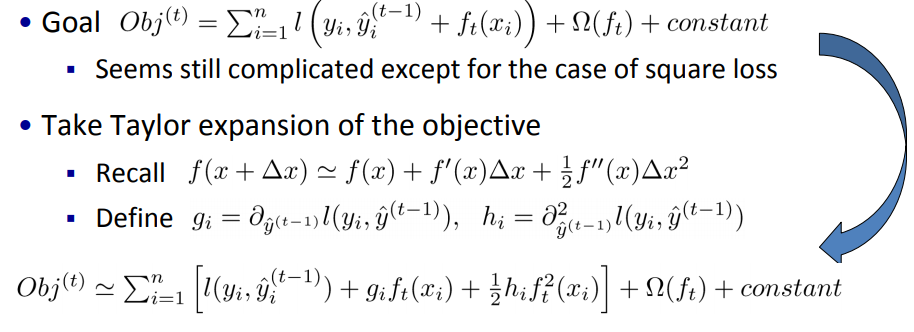
\includegraphics[width=4in,height=1.5in]{taylor}
\caption{}
\end{figure}

for detail see pdf in ml papers basis.

\textbf{lightgbm} choose the leaf with max delta loss to grow(leaf wise, best first), while most tree grow by level wise. Using max depth to control overfitting.

\section{GD, BGD, SGD, momentum, adagrad, adam}
GD refers to gradient descent, Using to negative gradient to optimize the ojbective function.
Batch gradient descent (BGD) computes the gradient on the whole dataset, which if often slow and intractable. Can not be applied to online model which data is on the fly. 
$$\theta=\theta - \eta \cdot \nabla_{\theta} J(\theta)$$
BGD guaranteed to converge to the global minimum for convex problem.

SGD perform an update for each training example. Usually slowly decrease the learning rate.
$$\theta=\theta - \eta \cdot \nabla_{\theta} J(\theta; x^{i};y^{i})$$

Mini-batch gradient descent perform an update for every mini batch of $n$ train examples. 

Momentum adagrad,adam, rmsprop etc are all opt strategy.

\section{EM Algorithm and VI}
In the topic of clustering, it can be classified as hard and soft clustering. EM is a soft clustering method which is a generative model which trys calculate parameters of probability distribution. 
EM algorithm is used for maximum likelihood estimates of parameters. In bayesian statistics, it is often used to obtain the mode of the posterior marginal distributions of parameters.

\textbf{E-step} computes the expected value of $l(\theta;X,Z)$ given the observed data $X$, and current estimate $\theta_{old}$.

\begin{align*}
Q(Z;\theta_{old}) &= P(Z| X,\theta_{old})
\end{align*}

\textbf{M-step} maximizing over $\theta$ the expectation computed.
\begin{align*}
\theta_{new} :&= \mathop{\arg\max}_{\theta} -KL(Q(Z) || P(Z|X,\theta)) \\
&= \mathop{\arg\max}_{\theta} \sum_{i}\sum_{z^{i}} Q_{i}(z^{i})log \frac{p(x^{i},z^{i};\theta)}{Q_{i}(z^{i})}
\end{align*}

In variational inference, we know that 
$$logp(x)=KL(q(z)||p(z|x))+(E_{q}[logp(z,x)]-E_{q}[logq(z)])$$
The difference of EM and VB is the kind of results they provide: \textbf{EM is just a point, VB is a distribution}. However, they also have similarities. EM and VB can both be interpreted as minimizing some sort of distance between the true value and our estimate, which is the Kullback-Leibler divergence. \\
For example:

When the Gaussian model involves latent variables and parameters only, Expectation Maximization is enough to solve the model. 

If, on top of the latent variables, the parameters becomes random with prior distributions, the Variational Inference (or Variational Bayes) method is used.

\section{Precision and Recall and F-measure and mAP}

\textbf{Accuracy}
\textbf{Precision}
\begin{itemize}
\item Meaningless, most case 99\% documents are none-relevant
\end{itemize}
$$Accuracy=\frac{TP+TN}{N}$$

\textbf{Precision}
\begin{itemize}
\item Intuition: how much junk did we give to the user ?
\end{itemize}
$$Precision=\frac{TP}{TP+FP}$$

\textbf{Recall}
\begin{itemize}
\item Intuition: how much good stuff did we miss ?
\end{itemize}
$$Recall=\frac{TP}{TP+FN}$$

\textbf{F-measure}
\begin{itemize}
\item Intuition: combine recall and precision
\end{itemize}
$$F_{\beta}=\frac{(\beta^{2}+1) \cdot P \cdot R}{\beta^{2}P+R}$$
$$F_{1}=\frac{2 \cdot P \cdot R}{P+R}$$

However, all of this may be misleading. They could be the same system.
\begin{figure}[H]
\centering
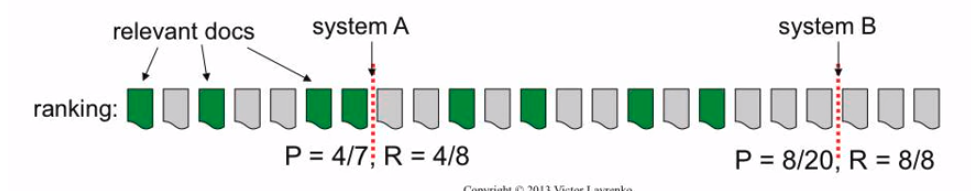
\includegraphics[width=5in,height=1in]{eval}
\caption{Same system, different score}
\end{figure}

Relationship between Recall/Precision/F1 in ranking:
\begin{figure}[H]
\centering
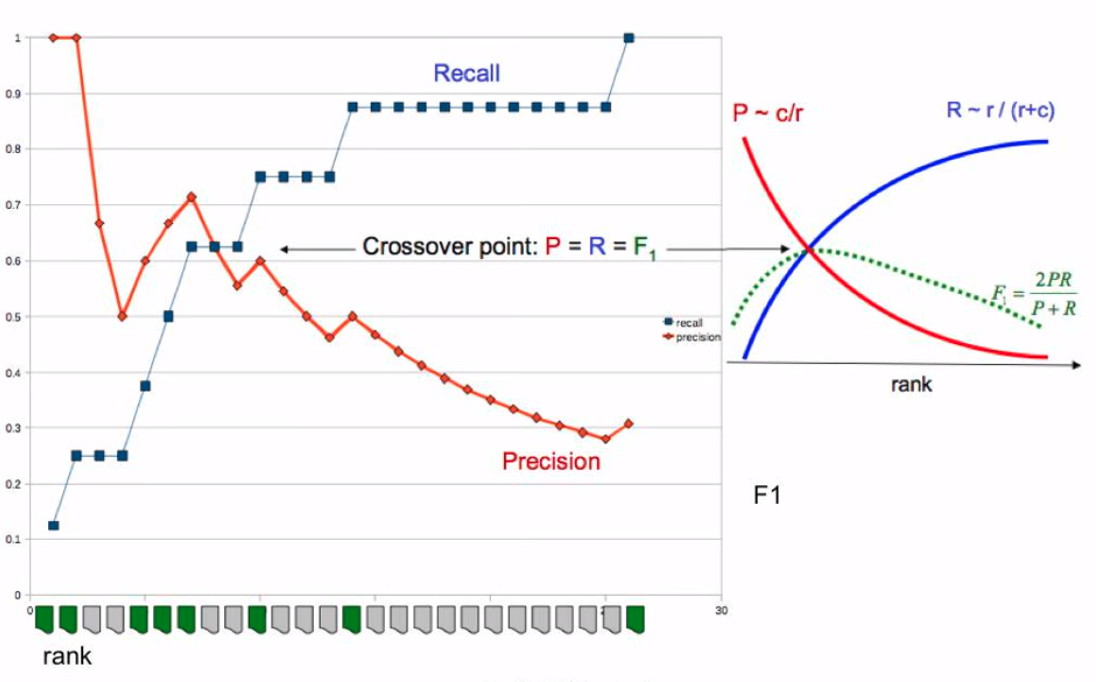
\includegraphics[width=4.5in,height=3in]{rank1}
\caption{Same system, different score}
\end{figure}

\textbf{Mean Average Precision}
\begin{itemize}
\item Assume user wants to find many relevant docs
\item biased towards top of the ranking (related with NDCG)
\end{itemize}
\begin{figure}[H]
\centering
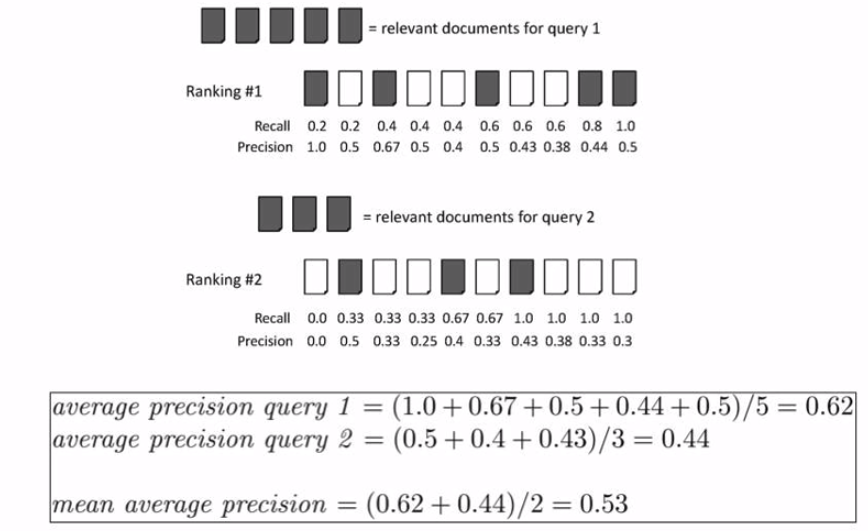
\includegraphics[width=5in,height=3in]{map}
\caption{mean average precision}
\end{figure}

\textbf{Normalized Discounted Cumulative Gain (NDCG)}

When we want none-binary metrics.
$$DCG_{k}=\sum_{r=1}^{k}\frac{rel_{r}}{log(r+1)}$$

\section{Learning to Rank}
\noindent
Pointwise
\\
Pairwise
\begin{itemize}
\item RankNet, RankSVM, RankBoost, GBRank
\end{itemize}
Listwise
\begin{itemize}
\item AdaRank, SoftRank, SVM-MAP, lambdaRank, lambdaMART
\end{itemize}

\section{SVM}
Ref: PRML / pluskid blog

For linear classification, we want to find a hyper plane:
$$w^{T}x+b=0$$
In SVM, we define functional margin as :
$$\widehat{\gamma}=y \cdot (w^{T}x+b) = yf(x) $$
Notice we multiply y to ensure $\widehat{\gamma} >0$
And we define geometrical margin as :
$$\widetilde{\gamma}= y \cdot \frac{w^{T}x+b}{||w||} = \frac{\widehat{\gamma}}{||w||} $$
The only difference between these two margin is the scale $||w||$. As the functional margin $\widehat{\gamma}$ can scaled by the $w$. 

In SVM, we want to find the best $w$ to maximize the margin. Here we can define $\widehat{\gamma}=1$, then we have our objective function:
$$max \frac{1}{||w||},\ s.t.,y_{i}(w^{T}x_{i}+b) \ge 1 $$
Which is equal to: 
$$min \frac{1}{2}||w||^{2},\ s.t.,y_{i}(w^{T}x_{i}+b) \ge 1 $$
This is a convex problem, we can apply \textbf{Lagrange multiplier}, convert the problem as:
$$L(w,b,\alpha)=\frac{1}{2}||w||^{2}-\sum_{i=1}^{n}\alpha_{i}(y_{i}(w^{T}x_{i}+b)-1)$$
$$\min \limits_{w,b}\theta(w)=\min \limits_{w,b} \max \limits_{\alpha_{i} \ge 0} L(w,b,\alpha)=p^{*} $$
It means that, when the condition meets, we want to find the best $w$ that minimize $\frac{1}{2}||w||^{2}$. 
Here we convert our objective to anther dual problem:
$$\max \limits_{\alpha_{i} \ge 0} \min \limits_{w,b}  L(w,b,\alpha) =d^{*} $$
as :
$$d^{*} \leq q^{*}$$ 
with $\partial L / \partial w =0 $, $\partial L / \partial b =0 $, we have:
$$L(w,b,\alpha)=\sum \alpha_{i}-\frac{1}{2}\sum \alpha_{i}\alpha_{j}y_{i}y_{j}x_{i}^{T}x_{j}$$
$$s.t., \alpha_{i} \ge 0, \sum \alpha_{i}y_{i}=0 $$

\textbf{Slack variable} means that svm allow some of noise vector inside the hyper-plane. specifically, we have:
$$y_{i}(w^{T}x_{i}+b) \ge 1 - \epsilon_{i}$$
And our new target is: 
$$min \frac{1}{2} ||w||^{2} +C\sum \epsilon_{i}$$
Same mathematics as above, we finally get: 
$$L(w,b,\alpha)=\sum \alpha_{i}-\frac{1}{2}\sum \alpha_{i}\alpha_{j}y_{i}y_{j}x_{i}^{T}x_{j}$$
$$s.t.,  0 \leq \alpha_{i} \leq C, \sum \alpha_{i}y_{i}=0 $$
Note the only difference now is that $\alpha$ has a upper limit $C$. 
\bibliographystyle{plain}
\bibliography{ref}

\end{CJK*}
\end{document}




















